\documentclass[usenames,dvipsnames,aspectratio=169]{beamer}
\usepackage{../common/cpp}

\title[OO Programozás - C++]{OO Programozás}
\subtitle{Operátor felültöltés, másolás és átalakítás}

\begin{document}

%1
\begin{frame}[plain]
  \titlepage
  \logoalul
\end{frame}

\section{Operátorok felültöltése}

\subsection{Műveletek közönséges tagfüggvényekkel}

\begin{frame}
    Jelenlegi legjobb tudásunk szerint készítsünk osztályt egy \hiv{\href{https://hu.wikipedia.org/wiki/Komplex_sz\%C3\%A1mok}{komplex szám}} tárolására és műveletek elvégzésére, azaz:
    \begin{itemize}
        \item tároljuk a szám valós és képzetes részét, 
        \item készítsünk konstruktorokat,
        \item getter/setter tagfüggvényeket,
        \item és olyan függvényeket, melyekkel komplex számok összeadhatók és szorozhatók!
    \end{itemize}
\end{frame}

\begin{frame}
    \begin{exampleblock}{\textattachfile{Complex1.h}{Complex1.h}}
        \scriptsize
        \lstinputlisting[language=C++,linerange={6-21},numbers=left,firstnumber=6]{Complex1.h}
    \end{exampleblock}
\end{frame}

\begin{frame}
    \begin{exampleblock}{\textattachfile{Complex1.h}{Complex1.h}}
        \scriptsize
        \lstinputlisting[language=C++,linerange={22-37},numbers=left,firstnumber=22]{Complex1.h}
    \end{exampleblock}
\end{frame}

\begin{frame}
    \begin{exampleblock}{\textattachfile{main1.cpp}{main1.cpp}}
        \lstinputlisting[language=C++,linerange={1-10},numbers=left,firstnumber=1]{main1.cpp}
    \end{exampleblock}
\end{frame}

\subsection{Felültöltött operátorok tagfüggvényekkel}

\begin{frame}
    Operátor felültöltés
    \begin{itemize}
        \item A C++ megengedi, hogy az operátorok jelentését kiterjesszük a saját típusainkra (osztályainkra)
        \item Pl. ha értelmezhető az összeadás két \texttt{int} vagy \texttt{float} között, akkor két \texttt{Complex} objektum miért ne lehetne összeadható?
        \item Az operátorok működését (praktikusan nyilvános tag)függvények adják meg $\to$ \texttt{operatorX}, ahol \texttt{X} pl. \texttt{+}, \texttt{*}.
    \end{itemize}
\end{frame}

\begin{frame}
    \begin{exampleblock}{\textattachfile{Complex2.h}{Complex2.h}}
        \scriptsize
        \lstinputlisting[language=C++,linerange={31-37},numbers=left,firstnumber=31]{Complex2.h}
    \end{exampleblock}
    \begin{itemize}
        \small
        \item $+$ művelet bal operandusa: aktuális objektum, a jobb oldalit paraméterként kapja.
        \item Utóbbi felesleges (tagonkénti) másolásának elkerülésére referenciát használunk.
        \item Új, ideiglenes (eredmény) objektum jön létre e kettő alapján, ezt adja vissza.
    \end{itemize}
\end{frame}

\begin{frame}
    \begin{exampleblock}{\textattachfile{main2.cpp}{main2.cpp}}
        \footnotesize
        \lstinputlisting[language=C++,linerange={4-16},numbers=left,firstnumber=4]{main2.cpp}
    \end{exampleblock}
\end{frame}

\begin{frame}
    \begin{description}[mm]
        \item[Probléma:] \hfill \\ Összeadásnál a jobb oldali operandusnak \texttt{Complex}-nek kell lennie.
        \item[Megoldás:] \hfill \\ További felültöltött operátor függvények hozzáadása, pl. \texttt{double}-t hozzáadhatunk a valós részhez.
    \end{description}
    \begin{exampleblock}{\textattachfile{Complex3.h}{Complex3.h}}
        \lstinputlisting[language=C++,linerange={35-37},numbers=left,firstnumber=32]{Complex3.h}
    \end{exampleblock}
\end{frame}

\begin{frame}
    \begin{exampleblock}{\textattachfile{main3.cpp}{main3.cpp}}
        \small
        \lstinputlisting[language=C++,linerange={4-14},numbers=left,firstnumber=4]{main3.cpp}
    \end{exampleblock}
\end{frame}

\subsection{Felültöltött operátorok barát függvényekkel}

\begin{frame}
    \begin{itemize}
        \item Ez sem segít, ha a \emph{bal} operandus \texttt{double} típusú $\to$ \emph{nem tag}, két paraméteres \texttt{operator} függvény.
        \item Nem éri el a privát/védett tagokat $\to$ barát (\texttt{friend}) függvény: mindenhez hozzáfér az osztályon belül.
        \item Másik osztály is lehet az osztályunk barátja, pl.: \\ \texttt{friend class FriendOfComplex;}
    \end{itemize}
\end{frame}

\begin{frame}
    \begin{exampleblock}{\textattachfile{Complex4.h}{Complex4.h}}
        \scriptsize
        \lstinputlisting[language=C++,linerange={6-8},numbers=left,firstnumber=6]{Complex4.h}
        \lstinputlisting[language=C++,linerange={28-36},numbers=left,firstnumber=28]{Complex4.h}
    \end{exampleblock}
\end{frame}

\begin{frame}
    \begin{exampleblock}{\textattachfile{Complex4.cpp}{Complex4.cpp}}
        \footnotesize
        \lstinputlisting[language=C++,linerange={3-10},numbers=left,firstnumber=3]{Complex4.cpp}
    \end{exampleblock}
\end{frame}

\begin{frame}
    \begin{exampleblock}{\textattachfile{main4.cpp}{main4.cpp}}
        \small
        \lstinputlisting[language=C++,linerange={4-14},numbers=left,firstnumber=4]{main4.cpp}
    \end{exampleblock}
\end{frame}

\begin{frame}
    Az \hiv{\href{https://cplusplus.com/reference/ostream/ostream/}{\texttt{ostream}}} a \texttt{cout}, \texttt{cerr} és \texttt{clog} objektumok típusa.
    \vfill
    \begin{center}
        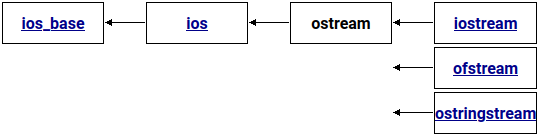
\includegraphics[scale=.5]{ostream.png}
    \end{center}
    \vfill
    Bár különösebb haszna nincs, de csupa nem tag barát függvénnyel is megoldhattuk volna az operátorok felültöltését.
\end{frame}

\begin{frame}
    \begin{exampleblock}{\textattachfile{Complex5.h}{Complex5.h} (\textattachfile{Complex5.cpp}{Complex5.cpp})}
        \scriptsize
        \lstinputlisting[language=C++,linerange={6-8},numbers=left,firstnumber=6]{Complex5.h}
        \lstinputlisting[language=C++,linerange={28-37},numbers=left,firstnumber=28]{Complex5.h}
    \end{exampleblock}
\end{frame}

\begin{frame}
    \hiv{\href{https://en.cppreference.com/w/cpp/language/operators}{Operátor felültöltés}}
    \begin{itemize}
        \item Definiáltuk az operátor \emph{jelentését} olyan kifejezésben, melyben legalább egy operandus az osztály objektuma.
        \item Nem változtatható meg az operátor \emph{szintakszisa}, \emph{precedenciája}, \emph{asszociativitása}, \emph{operandusainak száma}.
        \item \emph{Majdnem} minden operátor felültölthető.
    \end{itemize}
\end{frame}

\subsection{Az értékadás operátor felültöltése}

\begin{frame}
    \begin{itemize}
        \item Az értékadás megengedett objektumok között $\to$ tagonkénti másolás.
        \item Probléma: dinamikusan foglalt területet több objektum adattagja is címezhet. Ha az egyik destruktora ezt felszabadítja, a másik ezen próbálhat műveletet végezni vagy újra felszabadítani.
        \item Egészítsük ki a \textattachfile{../ea01/message.cpp}{Message} osztályt felültöltött értékadás operátorral, készítsünk másolatot a tárolt szövegről!
    \end{itemize}
\end{frame}

\begin{frame}
    \begin{exampleblock}{\textattachfile{message2.cpp}{message2.cpp}}
        \footnotesize
        \lstinputlisting[language=C++,linerange={4-17},numbers=left,firstnumber=4]{message2.cpp}
    \end{exampleblock}
\end{frame}

\begin{frame}
    \begin{exampleblock}{\textattachfile{message2.cpp}{message2.cpp}}
        \scriptsize
        \lstinputlisting[language=C++,linerange={19-32},numbers=left,firstnumber=19]{message2.cpp}
    \end{exampleblock}
\end{frame}

\begin{frame}
    \begin{exampleblock}{\textattachfile{message2.cpp}{message2.cpp}}
        \small
        \lstinputlisting[language=C++,linerange={34-44},numbers=left,firstnumber=34]{message2.cpp}
    \end{exampleblock}
\end{frame}

\begin{frame}[fragile]
    \begin{columns}[T]
        \column{.5\textwidth}
            \begin{exampleblock}{\textattachfile{message2.cpp}{message2.cpp}}
                \vspace{-.2cm}
                \fontsize{7}{8} \selectfont
                \lstinputlisting[language=C++,linerange={46-64},numbers=left,firstnumber=46]{message2.cpp}
                \vspace{-.2cm}
            \end{exampleblock}
        \column{.5\textwidth}
            \begin{block}{Kimenet}
                \vspace{-.4cm}
                \footnotesize
                \begin{verbatim}
Created [0x7ffcf5018618]
Hello C++ world!
Created [0x7ffcf5018620]
Hello C++ world!
Created [0x7ffcf5018628]
Hello C++ world!
Hello C++ world!
Hello C++ world!
Freed [0x7ffcf5018630, Hello C++ world!]
Freed [0x7ffcf5018628, Hello C++ world!]
Freed [0x7ffcf5018620, Hello C++ world!]
Freed [0x7ffcf5018618, ]
free(): double free detected in tcache 2
Aborted (core dumped)               
\end{verbatim}             
                \vspace{-.4cm}
            \end{block}
    \end{columns}
\end{frame}

\begin{frame}
    \begin{description}[m]
        \item[Ami jól működik:] \hfill \\ Az értékadás operátor, ami másolatot hoz létre a karakterláncból, \\nem engedi magát önmagára másolni, és \\a többszörös értékadás is működik a visszaadott referencia miatt.
        \item[Ami hibás:] \hfill \\ Az inicializáció nem értékadás, ilyenkor nem fut le a felültöltött függvényünk!
    \end{description}
\end{frame}

\section{Különleges konstruktorok}

\subsection{A másolási konstruktor}

\begin{frame}
    \begin{description}[m]
        \item[Másolási konstruktor (copy constructor):] \hfill \\ Akár \emph{egyetlen, azonos típusra vonatkozó referencia} paraméterrel is hívható konstruktor. (Lehetnek további paraméterek alapértelmezett értékekkel.)
        \item[Konverziós konstruktor (conversion constructor):] \hfill \\ Ez is hívható egyetlen paraméterrel, de az más típusú.
    \end{description}
    \vfill
    Közös tulajdonság: objektum \emph{inicializálásának} lehetősége kétféle szintaktikával: \\
    \texttt{Osztaly obj(42);} $\quad\equiv\quad$ \texttt{Osztaly obj = 42;} 
\end{frame}

\begin{frame}
    Másolási konstruktor további tulajdonságai:
    \begin{itemize}
        \item Ha mi nem készítünk, a fordító létrehoz egyet $\to$ tagonkénti másolás.
        \item Impliciten hívásra kerül:
            \begin{itemize}
                \item Objektum átadása függvénynek paraméterként $\to$ a végtelen rekurzió elkerülése miatt kell az első paraméternek referenciának lennie.
                \item Függvény adott osztály objektumát adja vissza.
            \end{itemize}
    \end{itemize}
\end{frame}

\begin{frame}
    \begin{exampleblock}{\textattachfile{message3.cpp}{message3.cpp}}
        \scriptsize
        \lstinputlisting[language=C++,linerange={13-27},numbers=left,firstnumber=13]{message3.cpp}
    \end{exampleblock}
\end{frame}

\begin{frame}[fragile]
    \begin{columns}[T]
        \column{.52\textwidth}
            \begin{exampleblock}{\textattachfile{message3.cpp}{message3.cpp}}
                \vspace{-.2cm}
                \scriptsize
                \lstinputlisting[language=C++,linerange={56-59},numbers=left,firstnumber=56]{message3.cpp}
                \lstinputlisting[language=C++,linerange={72-78},numbers=left,firstnumber=72]{message3.cpp}
                \vspace{-.2cm}
            \end{exampleblock}
        \column{.48\textwidth}
            \begin{block}{Kimenet}
                \vspace{-.4cm}
                \scriptsize
                \begin{verbatim}
Created [0x7fff0778e740]
Hello C++ world!
...
Created [0x7fff0778e758, Hello C++ world!]
Hello C++ world!
Created [0x7fff0778e760, Hello C++ world!]
Hello C++ world!
Created [0x7fff0778e768, Conversion ctor]
Created [0x7fff0778e770, Conversion ctor]
Freed [0x7fff0778e770, Conversion ctor]
Freed [0x7fff0778e768, Conversion ctor]
Freed [0x7fff0778e760, Hello C++ world!]
Freed [0x7fff0778e758, Hello C++ world!]
...
Freed [0x7fff0778e740, Hello C++ world!]
\end{verbatim}             
                \vspace{-.4cm}
            \end{block}
    \end{columns}
\end{frame}

\subsection{A konverziós konstruktor}

\begin{frame}
    Mikor hívjuk a konverziós konstruktort?
    \begin{itemize}
        \item Explicit hívás, más típusú adattal.
        \item Implicit hívás, a fordító egy adatot az osztály típusára akar alakítani $\to$ lehetővé teszi a felültöltött operátorfüggvények számának csökkentését!
    \end{itemize}
\end{frame}

\begin{frame}
    \begin{exampleblock}{\textattachfile{Complex6.h}{Complex6.h}}
        \scriptsize
        \lstinputlisting[language=C++,linerange={6-15},numbers=left,firstnumber=6]{Complex6.h}
        \lstinputlisting[language=C++,linerange={29-31},numbers=left,firstnumber=29]{Complex6.h}
    \end{exampleblock}
\end{frame}

\begin{frame}
    \begin{exampleblock}{\textattachfile{Complex6.h}{Complex6.h}}
        \scriptsize
        \lstinputlisting[language=C++,linerange={10-10},numbers=left,firstnumber=10]{Complex6.h}
    \end{exampleblock}
    \vfill
    Ha készítünk legalább egy konstruktort, a fordító nem hoz létre automatikusan \emph{alapértelmezett} konstruktort. Ha mégis szükség lenne rá: \texttt{default} \\ (C++11+; használható a kulcsszó más \emph{speciális} tagfüggvényekhez is.)
\end{frame}

\begin{frame}
    Legtöbbször ha szükség van az alábbiak közül akár csak egynek is a definiálására, akkor a másik kettőre is szükség van (\hiv{\href{https://en.wikipedia.org/wiki/Rule_of_three_(C\%2B\%2B_programming)}{Rule of Three}}):
    \begin{itemize}
        \item destruktor
        \item másoló konstruktor
        \item hozzárendelés operátor
    \end{itemize}
    \vfill
    Vagy, átmeneti jelleggel akár le is tilthatjuk egyes függvények alapértelmezett előállítását $\to$ \texttt{delete}\\
    Hasznos lehet nem kívánt típuskonverziók tiltására is.
\end{frame}

\begin{frame}
    \begin{exampleblock}{\textattachfile{message4.cpp}{message4.cpp}}
        \small
        \lstinputlisting[language=C++,linerange={4-4},numbers=left,firstnumber=4]{message4.cpp}
        \lstinputlisting[language=C++,linerange={7-7},numbers=left,firstnumber=7]{message4.cpp}
        \lstinputlisting[language=C++,linerange={19-20},numbers=left,firstnumber=19]{message4.cpp}
        \lstinputlisting[language=C++,linerange={29-30},numbers=left,firstnumber=29]{message4.cpp}
        \lstinputlisting[language=C++,linerange={37-37},numbers=left,firstnumber=37]{message4.cpp}
    \end{exampleblock}
\end{frame}

\begin{frame}
    \begin{exampleblock}{\textattachfile{message4.cpp}{message4.cpp}}
        \scriptsize
        \lstinputlisting[language=C++,linerange={44-44},numbers=left,firstnumber=44]{message4.cpp}
        \lstinputlisting[language=C++,linerange={49-61},numbers=left,firstnumber=49]{message4.cpp}
    \end{exampleblock}
\end{frame}

\end{document}